\documentclass[15pt,letterpaper]{article}
\usepackage{fullpage}
\usepackage[top=2cm, bottom=4.5cm, left=2.5cm, right=2.5cm]{geometry}
\usepackage{amsmath,amsthm,amsfonts,amssymb,amscd}
\usepackage{lastpage}
\usepackage{enumerate}
\usepackage{enumitem}
\usepackage{fancyhdr}
\usepackage{mathrsfs}
\usepackage{xcolor}
\usepackage{graphicx}
\usepackage{listings}
\usepackage{hyperref}
\usepackage{siunitx}
\usepackage{cancel}
\usepackage{caption}
\usepackage{subcaption}
\usepackage{wrapfig}

% mathcal
\newcommand{\Ac}{\mathcal{A}}
\newcommand{\Bc}{\mathcal{B}}
\newcommand{\Cc}{\mathcal{C}}
\newcommand{\Dc}{\mathcal{D}}
\newcommand{\Ec}{\mathcal{E}}
\newcommand{\Fc}{\mathcal{F}}
\newcommand{\Gc}{\mathcal{G}}
\newcommand{\Hc}{\mathcal{H}}
\newcommand{\Ic}{\mathcal{I}}
\newcommand{\Jc}{\mathcal{J}}
\newcommand{\Kc}{\mathcal{K}}
\newcommand{\Lc}{\mathcal{L}}
\newcommand{\Mc}{\mathcal{M}}
\newcommand{\Nc}{\mathcal{N}}
\newcommand{\Oc}{\mathcal{O}}
\newcommand{\Pc}{\mathcal{P}}
\newcommand{\Qc}{\mathcal{Q}}
\newcommand{\Rc}{\mathcal{R}}
\newcommand{\Sc}{\mathcal{S}}
\newcommand{\Tc}{\mathcal{T}}
\newcommand{\Uc}{\mathcal{U}}
\newcommand{\Vc}{\mathcal{V}}
\newcommand{\Wc}{\mathcal{W}}
\newcommand{\Xc}{\mathcal{X}}
\newcommand{\Yc}{\mathcal{Y}}
\newcommand{\Zc}{\mathcal{Z}}

% mathbb
\newcommand{\Ab}{\mathbb{A}}
\newcommand{\Bb}{\mathbb{B}}
\newcommand{\Cb}{\mathbb{C}}
\newcommand{\Db}{\mathbb{D}}
\newcommand{\Eb}{\mathbb{E}}
\newcommand{\Fb}{\mathbb{F}}
\newcommand{\Gb}{\mathbb{G}}
\newcommand{\Hb}{\mathbb{H}}
\newcommand{\Ib}{\mathbb{I}}
\newcommand{\Jb}{\mathbb{J}}
\newcommand{\Kb}{\mathbb{K}}
\newcommand{\Lb}{\mathbb{L}}
\newcommand{\Mb}{\mathbb{M}}
\newcommand{\Nb}{\mathbb{N}}
\newcommand{\Ob}{\mathbb{O}}
\newcommand{\Pb}{\mathbb{P}}
\newcommand{\Qb}{\mathbb{Q}}
\newcommand{\Rb}{\mathbb{R}}
\newcommand{\Sb}{\mathbb{S}}
\newcommand{\Tb}{\mathbb{T}}
\newcommand{\Ub}{\mathbb{U}}
\newcommand{\Vb}{\mathbb{V}}
\newcommand{\Wb}{\mathbb{W}}
\newcommand{\Xb}{\mathbb{X}}
\newcommand{\Yb}{\mathbb{Y}}
\newcommand{\Zb}{\mathbb{Z}}

% mathbf lowercase
\newcommand{\av}{\mathbf{a}}
\newcommand{\bv}{\mathbf{b}}
\newcommand{\cv}{\mathbf{c}}
\newcommand{\dv}{\mathbf{d}}
\newcommand{\ev}{\mathbf{e}}
\newcommand{\fv}{\mathbf{f}}
\newcommand{\gv}{\mathbf{g}}
\newcommand{\hv}{\mathbf{h}}
\newcommand{\iv}{\mathbf{i}}
\newcommand{\jv}{\mathbf{j}}
\newcommand{\kv}{\mathbf{k}}
\newcommand{\lv}{\mathbf{l}}
\newcommand{\mv}{\mathbf{m}}
\newcommand{\nv}{\mathbf{n}}
\newcommand{\ov}{\mathbf{o}}
\newcommand{\pv}{\mathbf{p}}
\newcommand{\qv}{\mathbf{q}}
\newcommand{\rv}{\mathbf{r}}
\newcommand{\sv}{\mathbf{s}}
\newcommand{\tv}{\mathbf{t}}
\newcommand{\uv}{\mathbf{u}}
\newcommand{\vv}{\mathbf{v}}
\newcommand{\wv}{\mathbf{w}}
\newcommand{\xv}{\mathbf{x}}
\newcommand{\yv}{\mathbf{y}}
\newcommand{\zv}{\mathbf{z}}

% mathbf uppercase
\newcommand{\Av}{\mathbf{A}}
\newcommand{\Bv}{\mathbf{B}}
\newcommand{\Cv}{\mathbf{C}}
\newcommand{\Dv}{\mathbf{D}}
\newcommand{\Ev}{\mathbf{E}}
\newcommand{\Fv}{\mathbf{F}}
\newcommand{\Gv}{\mathbf{G}}
\newcommand{\Hv}{\mathbf{H}}
\newcommand{\Iv}{\mathbf{I}}
\newcommand{\Jv}{\mathbf{J}}
\newcommand{\Kv}{\mathbf{K}}
\newcommand{\Lv}{\mathbf{L}}
\newcommand{\Mv}{\mathbf{M}}
\newcommand{\Nv}{\mathbf{N}}
\newcommand{\Ov}{\mathbf{O}}
\newcommand{\Pv}{\mathbf{P}}
\newcommand{\Qv}{\mathbf{Q}}
\newcommand{\Rv}{\mathbf{R}}
\newcommand{\Sv}{\mathbf{S}}
\newcommand{\Tv}{\mathbf{T}}
\newcommand{\Uv}{\mathbf{U}}
\newcommand{\Vv}{\mathbf{V}}
\newcommand{\Wv}{\mathbf{W}}
\newcommand{\Xv}{\mathbf{X}}
\newcommand{\Yv}{\mathbf{Y}}
\newcommand{\Zv}{\mathbf{Z}}

% bold greek lowercase
\newcommand{\alphav     }{\boldsymbol \alpha     }
\newcommand{\betav      }{\boldsymbol \beta      }
\newcommand{\gammav     }{\boldsymbol \gamma     }
\newcommand{\deltav     }{\boldsymbol \delta     }
\newcommand{\epsilonv   }{\boldsymbol \epsilon   }
\newcommand{\varepsilonv}{\boldsymbol \varepsilon}
\newcommand{\zetav      }{\boldsymbol \zeta      }
\newcommand{\etav       }{\boldsymbol \eta       }
\newcommand{\thetav     }{\boldsymbol \theta     }
\newcommand{\varthetav  }{\boldsymbol \vartheta  }
\newcommand{\iotav      }{\boldsymbol \iota      }
\newcommand{\kappav     }{\boldsymbol \kappa     }
\newcommand{\varkappav  }{\boldsymbol \varkappa  }
\newcommand{\lambdav    }{\boldsymbol \lambda    }
\newcommand{\muv        }{\boldsymbol \mu        }
\newcommand{\nuv        }{\boldsymbol \nu        }
\newcommand{\xiv        }{\boldsymbol \xi        }
\newcommand{\omicronv   }{\boldsymbol \omicron   }
\newcommand{\piv        }{\boldsymbol \pi        }
\newcommand{\varpiv     }{\boldsymbol \varpi     }
\newcommand{\rhov       }{\boldsymbol \rho       }
\newcommand{\varrhov    }{\boldsymbol \varrho    }
\newcommand{\sigmav     }{\boldsymbol \sigma     }
\newcommand{\varsigmav  }{\boldsymbol \varsigma  }
\newcommand{\tauv       }{\boldsymbol \tau       }
\newcommand{\upsilonv   }{\boldsymbol \upsilon   }
\newcommand{\phiv       }{\boldsymbol \phi       }
\newcommand{\varphiv    }{\boldsymbol \varphi    }
\newcommand{\chiv       }{\boldsymbol \chi       }
\newcommand{\psiv       }{\boldsymbol \psi       }
\newcommand{\omegav     }{\boldsymbol \omega     }

% bold greek uppercase
\newcommand{\Gammav     }{\boldsymbol \Gamma     }
\newcommand{\Deltav     }{\boldsymbol \Delta     }
\newcommand{\Thetav     }{\boldsymbol \Theta     }
\newcommand{\Lambdav    }{\boldsymbol \Lambda    }
\newcommand{\Xiv        }{\boldsymbol \Xi        }
\newcommand{\Piv        }{\boldsymbol \Pi        }
\newcommand{\Sigmav     }{\boldsymbol \Sigma     }
\newcommand{\Upsilonv   }{\boldsymbol \Upsilon   }
\newcommand{\Phiv       }{\boldsymbol \Phi       }
\newcommand{\Psiv       }{\boldsymbol \Psi       }
\newcommand{\Omegav     }{\boldsymbol \Omega     }

% Shortcut for user-defined commands
\newcommand{\todo}[1]{\textcolor{red}{TODO: #1}}

\hypersetup{%
  colorlinks=true,
  linkcolor=blue,
  linkbordercolor={0 0 1}
}

\renewcommand\lstlistingname{Algorithm}
\renewcommand\lstlistlistingname{Algorithms}
\def\lstlistingautorefname{Alg.}

\DeclareMathOperator*{\argmax}{arg\!\max}
\DeclareMathOperator*{\argmin}{arg\!\min}

\newcommand\scalemath[2]{\scalebox{#1}{\mbox{\ensuremath{\displaystyle #2}}}}
\newcommand{\norm}[1]{\left\lVert#1\right\rVert}

\newenvironment{amatrix}[1]{%
  \left(\begin{array}{@{}*{#1}{c}c@{}}
}{%
  \end{array}\right)
}

\definecolor{codegreen}{rgb}{0,0.6,0}
\definecolor{codegray}{rgb}{0.5,0.5,0.5}
\definecolor{codepurple}{rgb}{0.58,0,0.82}
\definecolor{backcolour}{rgb}{0.95,0.95,0.92}

\lstdefinestyle{mystyle}{
    language=C++,
    backgroundcolor=\color{backcolour},
    commentstyle=\color{codegreen},
    keywordstyle=\color{magenta},
    numberstyle=\tiny\color{codegray},
    stringstyle=\color{codepurple},
    basicstyle=\ttfamily\scriptsize,
    breakatwhitespace=false,
    breaklines=true,
    captionpos=b,
    keepspaces=true,
    numbers=left,
    numbersep=5pt,
    showspaces=false,
    showstringspaces=false,
    showtabs=false,
    tabsize=2
}

\lstset{style=mystyle}

\setlength{\parindent}{0.0in}
\setlength{\parskip}{0.05in}

% Edit these as appropriate
\newcommand\course{10708}
\newcommand\hwnumber{1}                  % <-- homework number
\newcommand\NetIDa{tkhurana \\ akashsha \\ eli1}           % <-- NetID of person #1

\pagestyle{fancyplain}
\headheight 35pt
\lhead{\NetIDa}                 % <-- Comment this line out for problem sets (make sure you are person #1)
\chead{Project Proposal}
\rhead{\course \\ \today}
\lfoot{}
\cfoot{}
\rfoot{\small\thepage}
\headsep 1.5em

\begin{document}

\section{Task, Dataset and Metrics}%
\label{sec:Task, Dataset and Metrics}
\textbf{Task:} For this project, we aim to cast the familiar robotics problem of Simultaneous Localization and Mapping (SLAM) as a dual optimization between the weights of a Multi-Layer Perceptron (MLP) that defines the \emph{map} and a sequence of 3D poses $T \in SE(3)$ that defines the camera \emph{trajectory} for a given scene. Our hope is to show that an implicit function representation of a scene via neural networks allows for scene completion that was not possible previously through geometric representations, and show that simultaneous optimization of the camera trajectory is feasible.

Consider a stream of incoming RGB frames (see Figure~\ref{fig:structured-prediction}). Each incoming frame associated with the 3D implicit function model via an unary consistency factor that can be defined through a rendering loss, and similarly between pairs of images, we define a new pairwise consistency factor, that enables us to formulate the problem as a structured prediction task of \emph{maximum a posteriori} estimation of the camera poses, while optimizing the scene.

\begin{wrapfigure}{l}{0.5\textwidth}
    \centering
    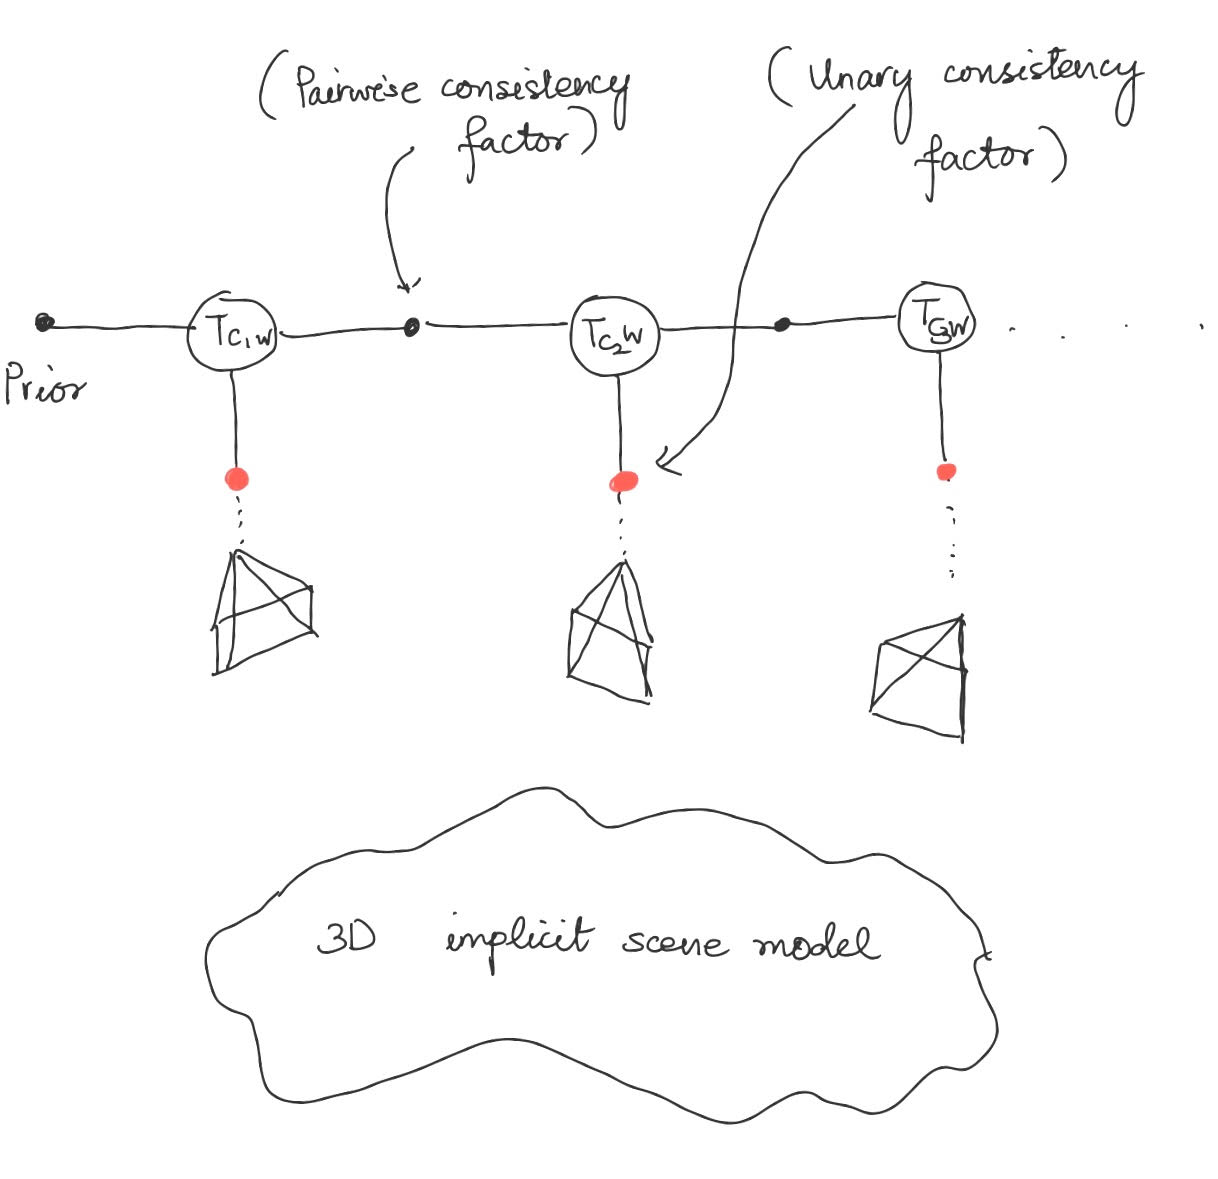
\includegraphics[width=\linewidth]{structured-prediction}
    \caption{Illustration of the problem formulation}%
    \label{fig:structured-prediction}
\end{wrapfigure}

\textbf{Dataset:} We will use the Replica dataset \cite{replica19arxiv} from Facebook Research for our task. The dataset includes a set of reconstructed indoor scenes with dense geometry. We will likely use the ReplicaRenderer to render images of the indoor scenes with a planned camera trajectory and feed \emph{unposed} images to the algorithm. Our fallback options for datasets are the Blender image dataset which comes with NeRF \cite{nerf} or the TUM RGBD dataset \cite{sturmBenchmarkEvaluationRGBD2012}.
{\bf Metrics:} We will measure the quality of novel view synthesis for the volumetric renderer via PSNR and SSIM. To quantitatively measure the accuracy of the 3D reconstruction we will measure the average distance of the points from the reconstructed scene and the ground truth. We will use standard Absolute trajectory error (ATE) metric, which measures the pose error for every camera pose in the trajectory against the ground truth. A more qualitative evaluation will be provided via visualization of the reconstructed scene and the optimized camera trajectory.

\textbf{Fallback Plan:} We will assume a pre-trained implicit funtion model of the scene, and given a sequence of unposed images, optimize over the pose variables through the differentiable renderer to generate relative pose measurements between the images. On obtaining these relative pose measurements, we can formulate the pose optimization as gaussian belief propagation over the pose graph (factor graph) to obtain the optimized camera poses.

\section{Approach}%
\label{sec:Approach}

We propose to solve the SLAM problem by building an implicit neural representation of a scene, encoded in the weights of an MLP, while also optimizing a sequence of camera poses for each incoming image in the RGB stream.

Specifically, in addition to the per pixel color loss used in NeRF (ref. Equation 1), we will impose per pixel color constraints between every pair of input images (ref. Equation 2). This is possible because every pair of images is associated with each other with a camera pose transformation which we want to optimize over.

\begin{align}
    l(\thetav, \Db) = \sum_{i = 1}^{K} \sum_{m,n = 1}^{N} C(r_i(m, n)) - \hat{C}(r_i(m,n))
\end{align}

\section{Related Work}%
\label{sec:Related Work}
{\bf SLAM:}
Simultaneous localization and mapping is a well researched problem which involves generating a map of a novel environment while tracking the agent's location within that environment. The key difficulties of the problem come from real time operation as this limits the amount of computation time and potential optimization complexity. ORB-SLAM \cite{orb_slam} provides a solution that not only operates in real time, but also maintains lifelong operation and deals with tracking failure. This efficiency is achieved by using ORB features for image matching for both mapping/tracking and place recognition \cite{orb}. Other approaches like DSO \cite{direct_odometry} avoid image feature mapping entirely and directly generate a local map by optimizing photometric error over a window of recent frames of the camera.

{\bf Graphical Models for SLAM:}
A novel method for solving the SLAM problem for large-scale environments introduces a Bayes Net representation where the agent's pose and landmark positions are recorded at various timesteps \cite{isam2}. These poses and positions represent nodes in the graph, and individual nodes are connected by directed edges from one timestep to the next and from the agent's pose to the position of a landmark. This reduces the problem to variable elimination, which works well given a small max clique size.

{\bf Implicit Scene Representation:}
Tangential to SLAM is the problem of scene reconstruction. Recently, this has been done implicitly by optimizing a neural radiance field representation for a complex scene \cite{nerf}. A neural radiance field representation models a 3 dimensional scene as a compilation of points sampled along camera rays shot from pixel locations of an image at a novel pose. These samples are represented as 5D coordinates (location and viewing direction), and are transformed using a neural network to estimate the color (i.e. shade, brightness, etc.) at those pixels.

This idea has been used recently for SLAM \cite{imap} where, given an RGB-D camera stream, a scene (including its unseen regions) can be mapped alongside predicting the camera trajectory from a small number of keypoint frames. In this work, we will attempt to do the same but without assuming access to depth sensors.

\section{Expected Outcomes}%
\label{sec:Expected Outcomes}
% \begin{enumerate}
%     \item A method that can learn scene geometry encoded in the network weights, and also optimize the camera trajectory simultaneously, given only RGB image stream
% \end{enumerate}
We expect to recover camera poses for RGB images in the incoming unposed camera stream. We also expect to simultaneously represent the 3D scene in the RGB images as a set of weights of a Multi-Layer Perceptron.

For these two end outcomes, we expect to tune the number of past RGB images required to compute the pairwise consistency loss terms. In addition to this, we will also hand-tune the number of pixels to render the scene representation at, per incoming image, so that we do not run out of compute. With the resources available to us, we hope to take a step towards solving this important and exciting task but do not commit to extraordinary results.
\section{Plan}%
\label{sec:Plan}

We will first need to set up the open-source NeRF codebase available at \hyperlink{https://github.com/bmild/nerf}{https://github.com/bmild/nerf} to use the baseline MLP architecture and volumetric rendering utilities. We will build on this codebase to incorporate our pairwise consistency criteria and build a factor graph to alternate between its and the MLP's optimization. This will require us to use the lietorch codebase too. We will additionally be generating our image dataset using the Renderer from the Replica dataset available at \hyperlink{https://github.com/facebookresearch/Replica-Dataset}{https://github.com/facebookresearch/Replica-Dataset}.

Eric will take on the task of curating the dataset which will be used by Tarasha to optimize the MLP weights and learn the poses. Akash will be responsible for the qualitative and quantitative evaluation.

\footnotesize

\bibliographystyle{abbrv}
\bibliography{references, references_zotero}

\end{document}

